\documentclass{article}
\usepackage{animate}
\usepackage{listings}
\usepackage{float}
% Language setting
% Replace `english' with e.g. `spanish' to change the document language
\usepackage[english]{babel}

% Set page size and margins
% Replace `letterpaper' with `a4paper' for UK/EU standard size
\usepackage[letterpaper,top=2cm,bottom=2cm,left=3cm,right=3cm,marginparwidth=1.75cm]{geometry}

% Useful packages
\usepackage{amsmath}
\usepackage{graphicx}
\usepackage[colorlinks=true, allcolors=blue]{hyperref}

\title{HAMS1K: Hardware Accelerated Merge Sort for sorting array of 1024 integers}
\author{Gaurav Dubey, Michael Salek}

\begin{document}
\maketitle

\begin{abstract}
In this paper, we present HAMS1K, a very basic hardware accelerated sorting algorithm designed to sort a 1024 integer input array. The implemented algorithm divides an unsorted array of 1024 integers into 256 sublists of 4 integers each. These 256 sublists are then sorted using a bitonic sort hardware implementation. Later hardware employs a parallel merge tree to repeatedly merge sublists until only one sublist remains. This sublist corresponds to the desired sorted list. This hardware implementation can only sort 1024 integers in its current form, but with some changes and a supporting application software, any unsorted array can be sorted. 
\end{abstract}

\section{Introduction}

Sorting is used in a variety of applications that deal with large amounts of data. Computers are processing more data than ever before thanks to cloud computing, machine learning, artificial intelligence, and the internet of things. As Moore's law slows, there is concern that the increase in compute resources will not be enough to meet the demand for compute resources to handle data that grows exponentially every year.

Sorting data involves subtasks such as comparing and swapping two integers. A simple swap function in C/C++ can be written in as few as four statements, as shown below, but this does not imply that the computer will execute it in four instructions. If we look at the disassembled code of the swap function below, we can see that the C/C++ compiler added a few more instructions to allow the machine to produce the desired results. These additional inserted instructions are required and consume a substantial number of compute time. In addition, there may be cases where the swap function is called for a variable involving cache misses, which will increase the execution time even more. 


\begin{lstlisting}
C/C++ code:
void swap(int * i, int *j) {
  int a = *i;   int b = *j;
  *i = b;   *j = a;
}

assembly:
swap:
      pushl %ebp          #setup, push data on stack for swap
      movl  %esp,%ebp     #setup
      pushl %ebx          #setup, push data on stack for swap
      movl  8(%ebp),%edx  #edx = i
      movl  12(%ebp),%ecx #ecx = j
      movl  (%edx),%ebx   #ebx = *i
      movl  (%ecx),%eax   #ecx = *j
      movl  %eax,(%edx)   #*i = b
      movl  %ebx,(%ecx)   #*j = a
      popl  %ebx          #finish, remove data from stack
      popl  %ebp          #finish, remove data from stack
      ret                 #finish
\end{lstlisting}

Compare and swap is quite expensive and so, sorting large amounts of data consumes significant compute resources.  Dedicated hardware for this problem can swap two variables in just 1 machine cycle and there is a growing interest in reducing this time by designing application-specific solutions to accelerate sorting algorithms in hardware. HAMS1K is one such attempt to speed up merge sorting through parallelism and locality.

HAMS1K includes RAMs to store data locally to avoid large memory read and write accesses latency. The hardware implementation consists of multiple RAMs, read and write accesses are performed in a manner that parallel merge tree can operate at optimal rates to speed up sorting.  



\section{Background}

\subsection{Merge Sort: serial implementation}

Merge Sort is a Divide and Conquer algorithm. Implementation of this algorithm involves three steps i.e. divide, conquer and merge.

The algorithm divides the input array into two sublists, then it separates these two sublists into four sublists, this process is continued until the lists are broken down until they can no longer be divided, leaving N sublists with just 1 element each, these N sublists can be considered as sorted. Here N is the length of the input array to be sorted.
Once these lists cannot be broken down further, it starts merging these N sublists such that merged lists are sorted in a particular order (say ascending order), conquering sort problem one step at a time. This process is illustrated in the figure \ref{fig:merge_serial}.

\begin{figure}[H]
\centering
  \animategraphics[loop,controls,width=\linewidth]{1}{merge_serial}{1}{9}
\caption{\label{fig:merge_serial}Illustration of the Merge sort algorithm.}
\end{figure}

The serial merge sort algorithm can be implemented in hardware by using a network (FIFO merge) of circular buffers, as shown in figure \ref{fig:fifo_nwk}. Because the algorithm divides the input array first, an array with N elements will have N sorted sublists. We use the FIFO merge to combine sorted N sublists into N/2 sorted lists with 2 elements. Then we combine N/2 sorted lists to make N/4 sorted lists, each with four elements. This process is repeated until we have a list of N elements.


\begin{figure}[H]
\centering
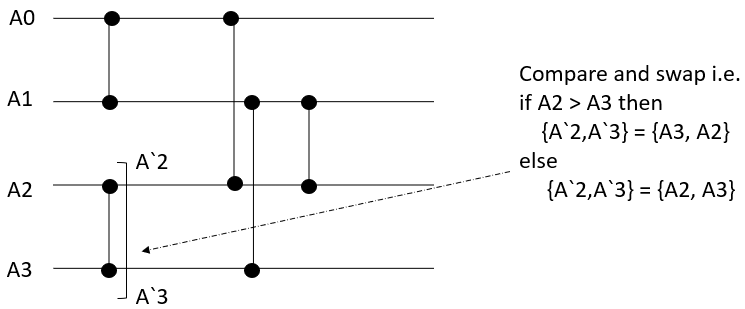
\includegraphics[width=1.00\textwidth]{fifo_nwk.PNG}
\caption{\label{fig:fifo_nwk}A hardware oriented design to merge two sorted list.}
\end{figure}


The hardware implementation will take 2N*$log_2N$ clock cycles to complete the sorting of the input array because the merging process is repeated $log_2N$ times, with each merging cycle requiring N clock cycles to read data and N clock cycles to write the merged sorted list back to memory.


\begin{figure}[H]
\centering
  \animategraphics[loop,controls,width=\linewidth]{1}{address_serial}{1}{33}
\caption{\label{fig:address_serial}Illustration of hardware implementation of serial Merge sort algorithm.}
\end{figure}


\begin{figure}[H]
\centering
%\embedvideo{\includegraphics[page=1]{example-movie}}{Rd1ElemAtATime.avi}
%\begin{frame}{Reading 1 key per clock}
  \animategraphics[loop,controls,width=\linewidth]{1}{ad-}{1}{8}
%\end{frame}

\caption{\label{fig:serial}This frog was uploaded via the file-tree menu.}
\end{figure}

\subsection{Bitonic Sort}

First you have to upload the image file from your computer using the upload link in the file-tree menu. Then use the includegraphics command to include it in your document. Use the figure environment and the caption command to add a number and a caption to your figure. %See the code for Figure \ref{fig:frog} in this section for an example.

Note that your figure will automatically be placed in the most appropriate place for it, given the surrounding text and taking into account other figures or tables that may be close by. You can find out more about adding images to your documents in this help article on \href{https://www.overleaf.com/learn/how-to/Including_images_on_Overleaf}{including images on Overleaf}.


\subsection{Merge Sort: parallel implementation}

Simply use the section and subsection commands, as in this example document! With Overleaf, all the formatting and numbering is handled automatically according to the template you've chosen. If you're using Rich Text mode, you can also create new section and subsections via the buttons in the editor toolbar.


\begin{figure}
\centering
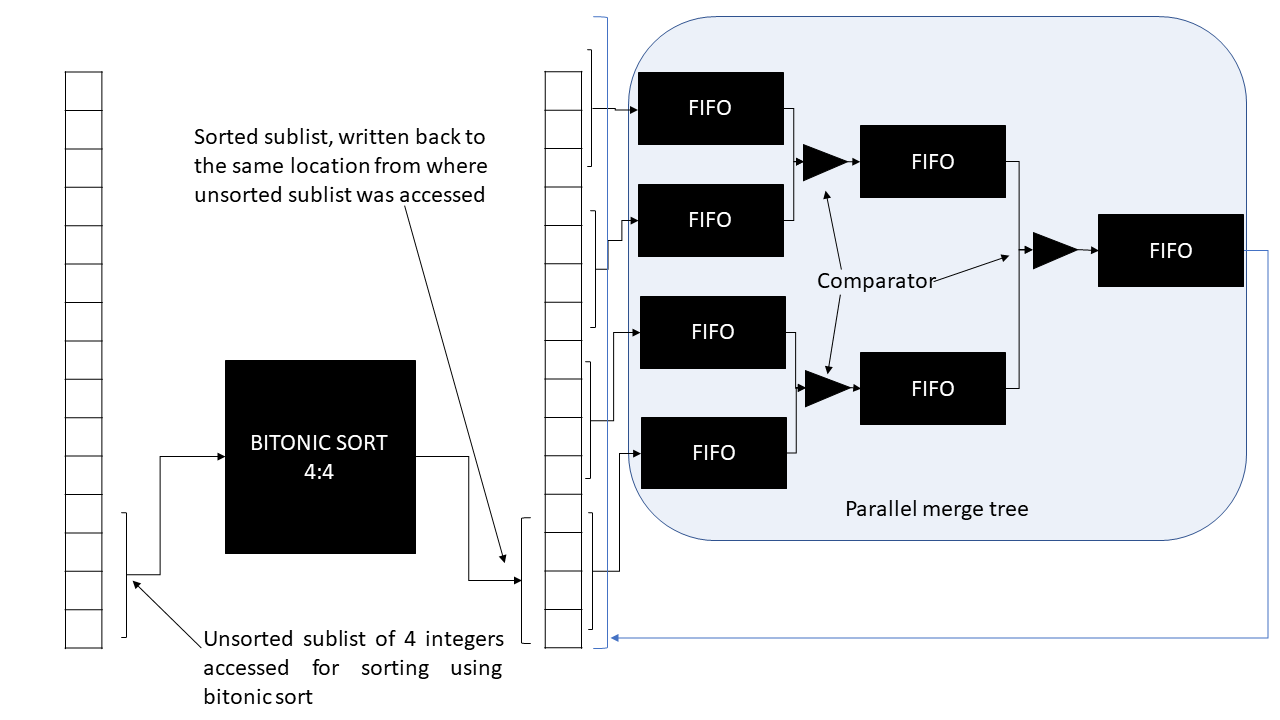
\includegraphics[width=1.00\textwidth]{hams_scheme.png}
\caption{\label{fig:scheme}Block diagram of HAMS1K hardware.}
\end{figure}


\subsection{How to add Tables}

Use the table and tabular environments for basic tables --- see Table~\ref{tab:widgets}, for example. For more information, please see this help article on \href{https://www.overleaf.com/learn/latex/tables}{tables}. 

\begin{table}
\centering
\begin{tabular}{l|r}
Item & Quantity \\\hline
Widgets & 42 \\
Gadgets & 13
\end{tabular}
\caption{\label{tab:widgets}An example table.}
\end{table}

\subsection{How to add Comments and Track Changes}

Comments can be added to your project by highlighting some text and clicking ``Add comment'' in the top right of the editor pane. To view existing comments, click on the Review menu in the toolbar above. To reply to a comment, click on the Reply button in the lower right corner of the comment. You can close the Review pane by clicking its name on the toolbar when you're done reviewing for the time being.

Track changes are available on all our \href{https://www.overleaf.com/user/subscription/plans}{premium plans}, and can be toggled on or off using the option at the top of the Review pane. Track changes allow you to keep track of every change made to the document, along with the person making the change. 

\subsection{How to add Lists}

You can make lists with automatic numbering \dots

\begin{enumerate}
\item Like this,
\item and like this.
\end{enumerate}
\dots or bullet points \dots
\begin{itemize}
\item Like this,
\item and like this.
\end{itemize}

\subsection{How to write Mathematics}

\LaTeX{} is great at typesetting mathematics. Let $X_1, X_2, \ldots, X_n$ be a sequence of independent and identically distributed random variables with $\text{E}[X_i] = \mu$ and $\text{Var}[X_i] = \sigma^2 < \infty$, and let
\[S_n = \frac{X_1 + X_2 + \cdots + X_n}{n}
      = \frac{1}{n}\sum_{i}^{n} X_i\]
denote their mean. Then as $n$ approaches infinity, the random variables $\sqrt{n}(S_n - \mu)$ converge in distribution to a normal $\mathcal{N}(0, \sigma^2)$.


\subsection{How to change the margins and paper size}

Usually the template you're using will have the page margins and paper size set correctly for that use-case. For example, if you're using a journal article template provided by the journal publisher, that template will be formatted according to their requirements. In these cases, it's best not to alter the margins directly.

If however you're using a more general template, such as this one, and would like to alter the margins, a common way to do so is via the geometry package. You can find the geometry package loaded in the preamble at the top of this example file, and if you'd like to learn more about how to adjust the settings, please visit this help article on \href{https://www.overleaf.com/learn/latex/page_size_and_margins}{page size and margins}.

\subsection{How to change the document language and spell check settings}

Overleaf supports many different languages, including multiple different languages within one document. 

To configure the document language, simply edit the option provided to the babel package in the preamble at the top of this example project. To learn more about the different options, please visit this help article on \href{https://www.overleaf.com/learn/latex/International_language_support}{international language support}.

To change the spell check language, simply open the Overleaf menu at the top left of the editor window, scroll down to the spell check setting, and adjust accordingly.

\subsection{How to add Citations and a References List}

You can simply upload a \verb|.bib| file containing your BibTeX entries, created with a tool such as JabRef. You can then cite entries from it, like this: \cite{greenwade93}. Just remember to specify a bibliography style, as well as the filename of the \verb|.bib|. You can find a \href{https://www.overleaf.com/help/97-how-to-include-a-bibliography-using-bibtex}{video tutorial here} to learn more about BibTeX.

If you have an \href{https://www.overleaf.com/user/subscription/plans}{upgraded account}, you can also import your Mendeley or Zotero library directly as a \verb|.bib| file, via the upload menu in the file-tree.

\subsection{Good luck!}

We hope you find Overleaf useful, and do take a look at our \href{https://www.overleaf.com/learn}{help library} for more tutorials and user guides! Please also let us know if you have any feedback using the Contact Us link at the bottom of the Overleaf menu --- or use the contact form at \url{https://www.overleaf.com/contact}.

\bibliographystyle{alpha}
\bibliography{sample}

\end{document}
